%%%%%%%%%%%%%%%%%%%%%%%%%%%%%%%%%%%%%%%%%%%%%%%%%%%%%%%%%%%%%%%%%%%%%%%%%%%%%%%%%%%%%%%%%%
\setcounter{section}{2}
\section{Manual Mode}

\subsection{First steps}

{\em Karel is returning from a long walk and his batteries are running out. 
Use the buttons on the left to get him home quickly! }
\begin{figure}[!ht]
\begin{center}
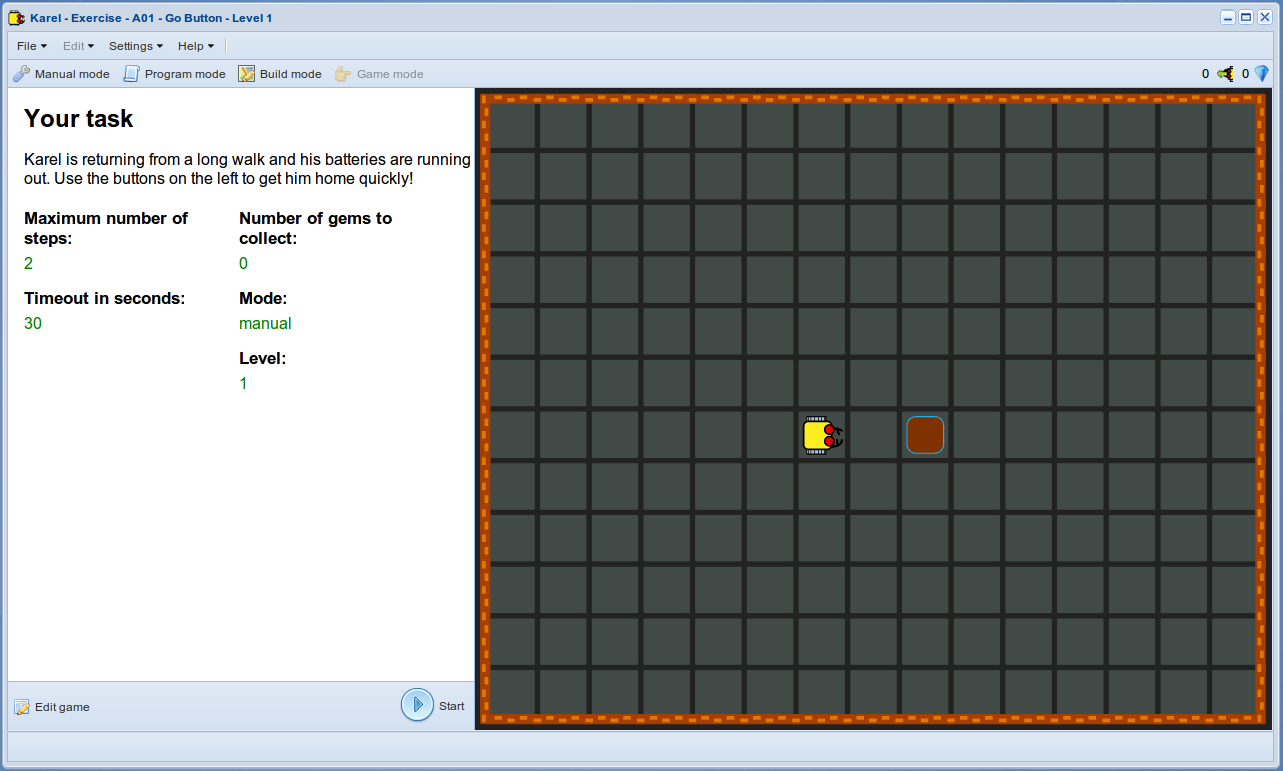
\includegraphics[height=0.4\textwidth]{img/a01.png}
\end{center}
\vspace{-4mm}
\caption{In the first exercise you need to help the robot get home.}
\label{fig:a01}
\end{figure}

\noindent
Pressing Start will start 
the exercise, and at this time also the buttons Go, Left, Right, Put and Get appear, 
as shown in Fig. \ref{fig:a01b}.


\begin{figure}[!ht]
\begin{center}
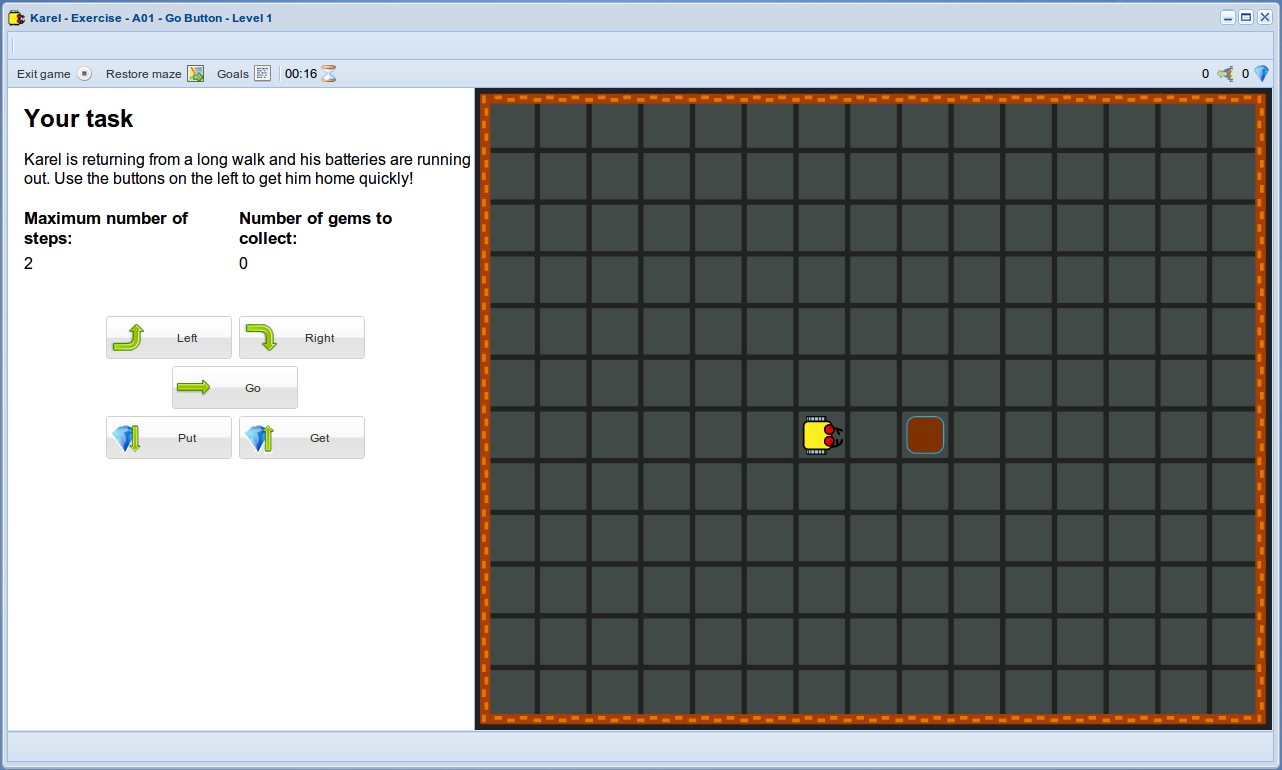
\includegraphics[height=0.4\textwidth]{img/a01b.png}
\end{center}
\vspace{-4mm}
\caption{Karel can be guided manually, using five buttons located in the left panel.}
\label{fig:a01b}
\vspace{-10mm}
\end{figure}

\newpage
\subsection{1st olympic games}

{\em Karel is training for Robolympic Games! Your task is to run with 
the robot home as fast as possible. Karel's personal record is four seconds. How fast can you be?}

\begin{figure}[!ht]
\begin{center}
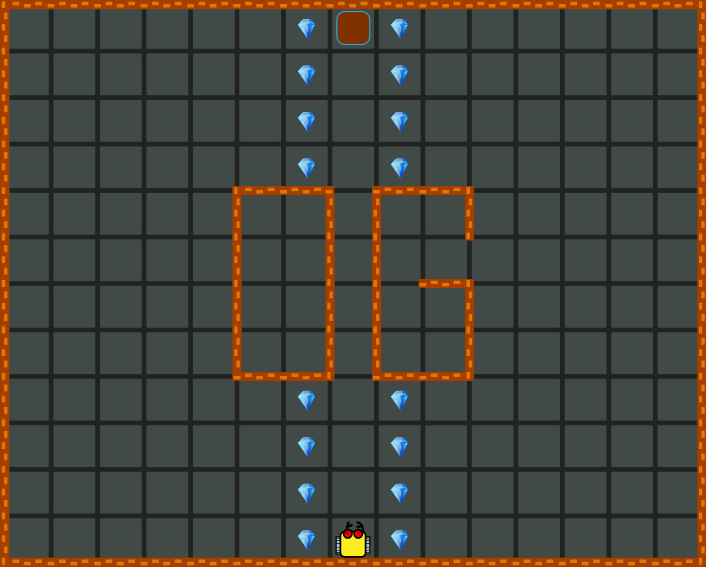
\includegraphics[height=0.4\textwidth]{img/a02.png}
\end{center}
\vspace{-4mm}
\caption{Karel is training for Robolympic Games.}
\label{fig:a02}
\vspace{-4mm}
\end{figure}
\noindent

\subsection{First gem}

{\em Today is Karel's lucky day because he is about to find his first gem. 
Use the buttons on the left to help the robot pick up the gem and carry it 
home!}

\begin{figure}[!ht]
\begin{center}
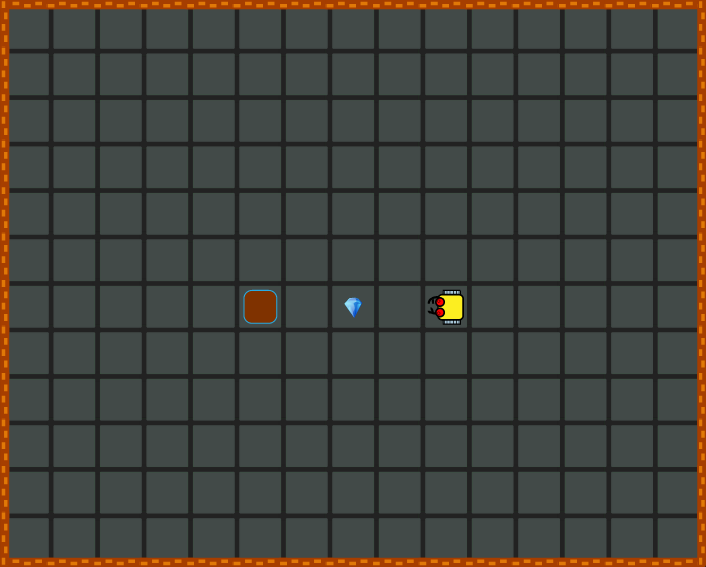
\includegraphics[height=0.4\textwidth]{img/a03.png}
\end{center}
\vspace{-4mm}
\caption{Karel is about to find his first gem.}
\label{fig:a03}
\vspace{-1cm}
\end{figure}
\noindent

\subsection{2nd olympic games}

{\em It is Robolympic season again! Run home as fast as you can, 
and collect all three gems on the way! Karel's personal record is 10 seconds.}


\begin{figure}[!ht]
\begin{center}
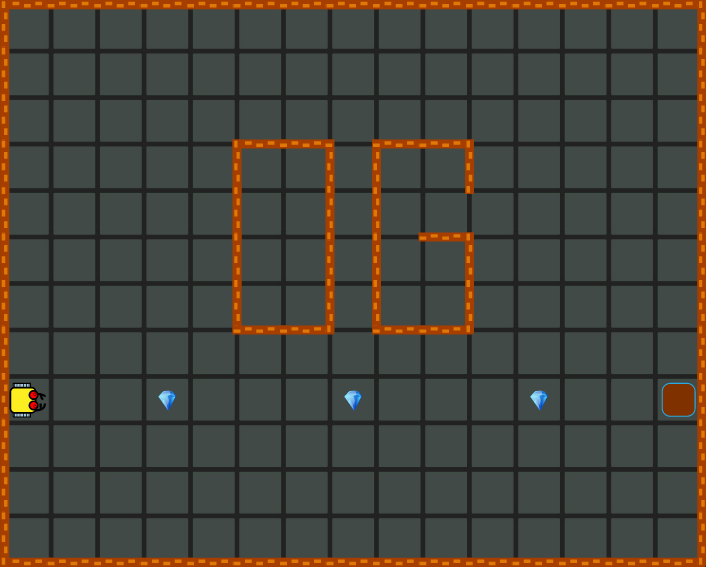
\includegraphics[height=0.4\textwidth]{img/a04.png}
\end{center}
\vspace{-4mm}
\caption{Karel's second Robolympic Games.}
\label{fig:a04}
\vspace{-1cm}
\end{figure}
\noindent


\subsection{First turn}

{\em Help the robot collect the gem and return home!}

\begin{figure}[!ht]
\begin{center}
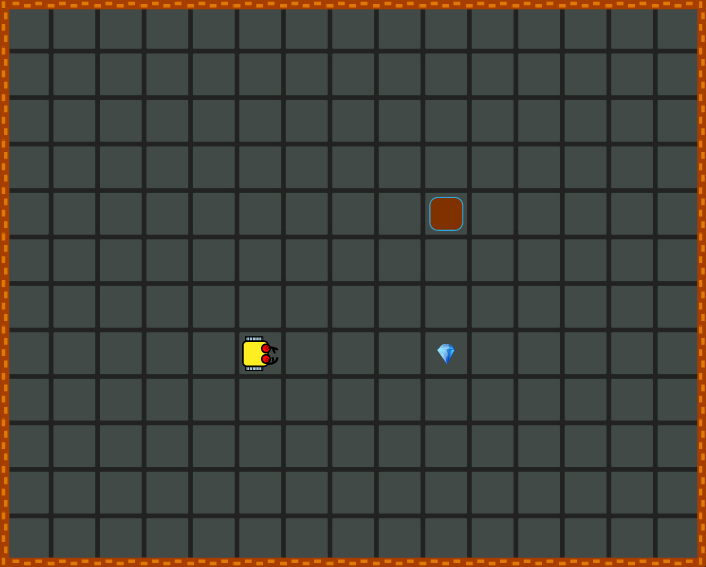
\includegraphics[height=0.4\textwidth]{img/a05.png}
\end{center}
\vspace{-4mm}
\caption{Karel is about to learn how to make a left turn.}
\label{fig:a05}
\vspace{-1cm}
\end{figure}
\noindent


\subsection{3rd olympic games}

{\em Karel is training for his third Robolympic Games. Run with him around the block and home as fast as possible. He needs to collect at least one gem on the way. Karel's personal record is 16 seconds!}

\begin{figure}[!ht]
\begin{center}
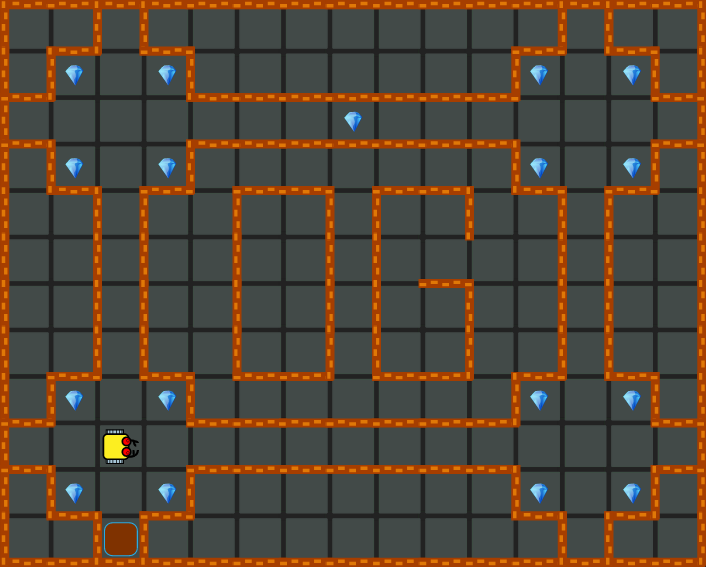
\includegraphics[height=0.4\textwidth]{img/a06.png}
\end{center}
\vspace{-4mm}
\caption{Karel's third Robolympic Games.}
\label{fig:a06}
\vspace{-1cm}
\end{figure}
\noindent


\subsection{Two gems}

{\em Pick up the two gems and get Karel home!}

\begin{figure}[!ht]
\begin{center}
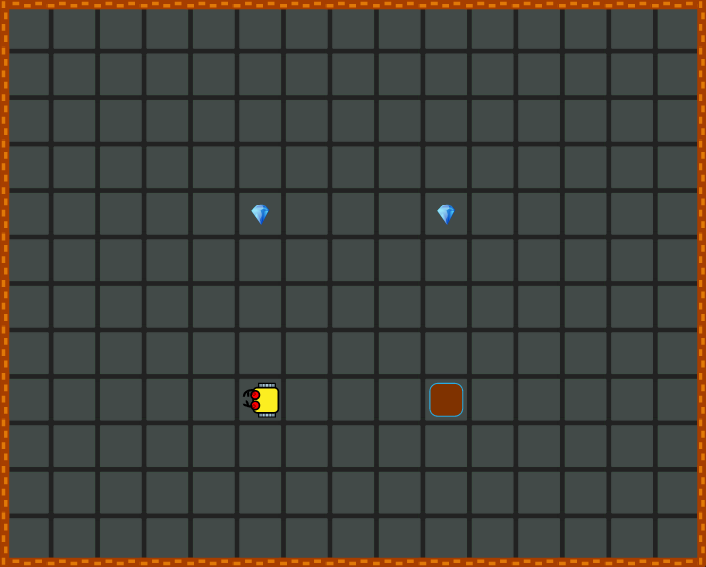
\includegraphics[height=0.4\textwidth]{img/a07.png}
\end{center}
\vspace{-4mm}
\caption{Karel needs to collect two gems and get home.}
\label{fig:a07}
\vspace{-1cm}
\end{figure}
\noindent

\subsection{4th olympic games}

{\em Last season of Karel's Robolympics Games is here! The 
robot needs to run home as fast as possible and bring one gem. 
Be careful not to crash, this is a tricky level! Karel's personal record is 26 seconds.}\\[-7mm]

\begin{figure}[!ht]
\begin{center}
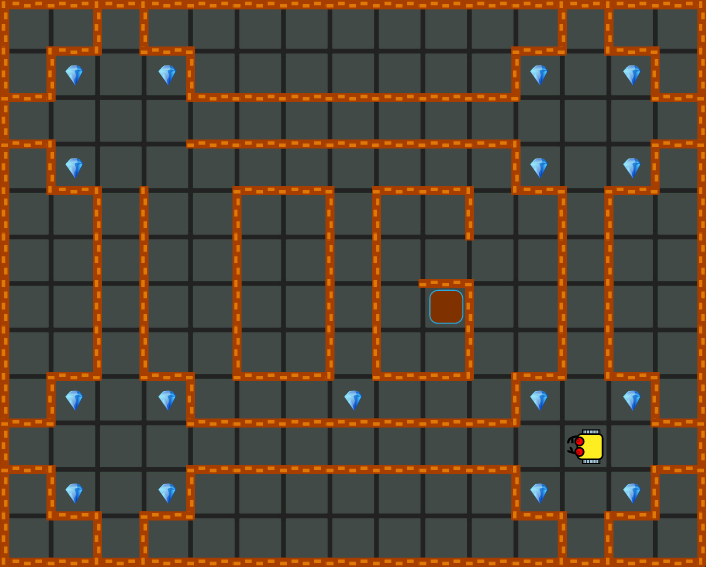
\includegraphics[height=0.4\textwidth]{img/a08.png}
\end{center}
\vspace{-4mm}
\caption{Karel's fourth Robolympic Games.}
\label{fig:a08}
\vspace{-4mm}
\end{figure}
\noindent

\subsection{Five gems}

{\em Help Karel collect five gems and get home!}\\[-7mm]

\begin{figure}[!ht]
\begin{center}
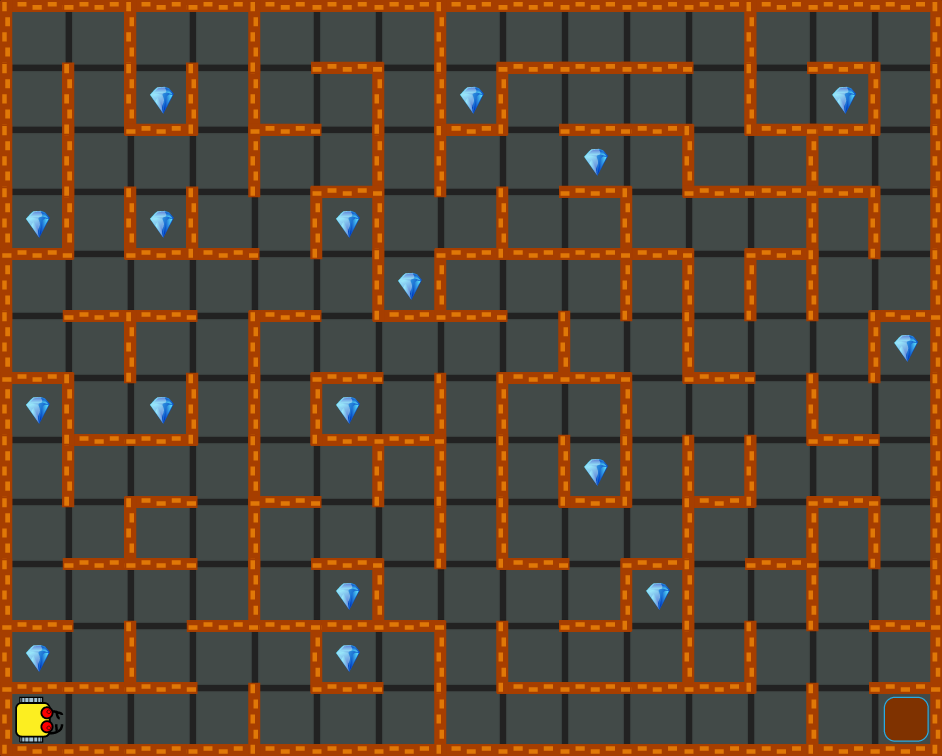
\includegraphics[height=0.4\textwidth]{img/a09.png}
\end{center}
\vspace{-4mm}
\caption{Karel needs to collect five gems.}
\label{fig:a09}
\vspace{-10mm}
\end{figure}
\noindent
\newpage

\subsection{Labyrinth}

{\em This is a true labyrinth and your task is to lead Karel 
home. Remember - think first before going anywhere!}

\begin{figure}[!ht]
\begin{center}
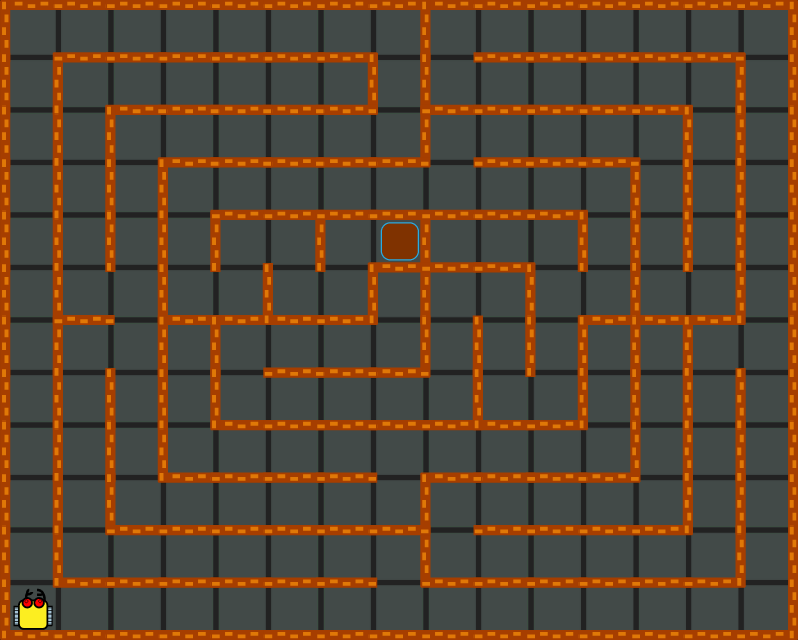
\includegraphics[height=0.4\textwidth]{img/a10.png}
\end{center}
\vspace{-4mm}
\caption{Karel needs to find his way home in a labyrinth.}
\label{fig:a10}
\vspace{-4mm}
\end{figure}
\noindent


\subsection{Diamond mine}

{\em Karel discovered an abandoned diamond mine. Use the buttons
on the left to collect all gems and get back home in time!}

\begin{figure}[!ht]
\begin{center}
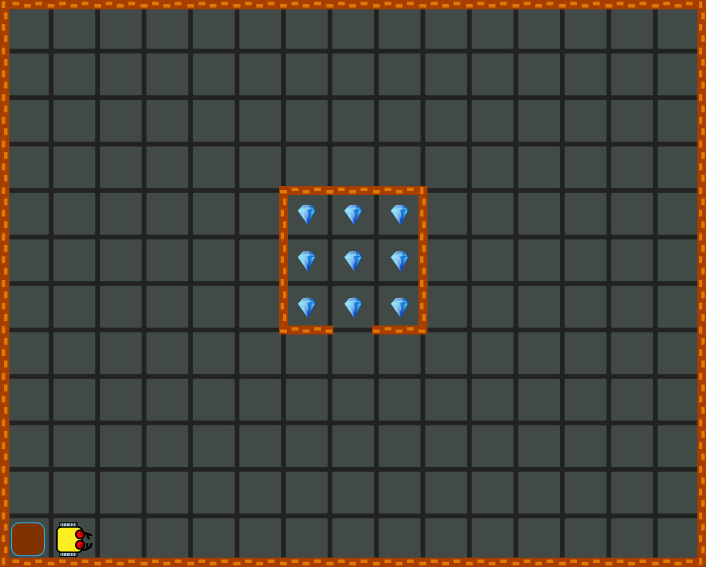
\includegraphics[height=0.4\textwidth]{img/a11.png}
\end{center}
\vspace{-4mm}
\caption{Karel found an abandoned diamond mine.}
\label{fig:a11}
\vspace{-10mm}
\end{figure}
\newpage
\noindent

\subsection{Piles of gems}

{\em If gems are piled up, then a number is showing their amount. 
Help Karel collect all gems in this maze and return home!}

\begin{figure}[!ht]
\begin{center}
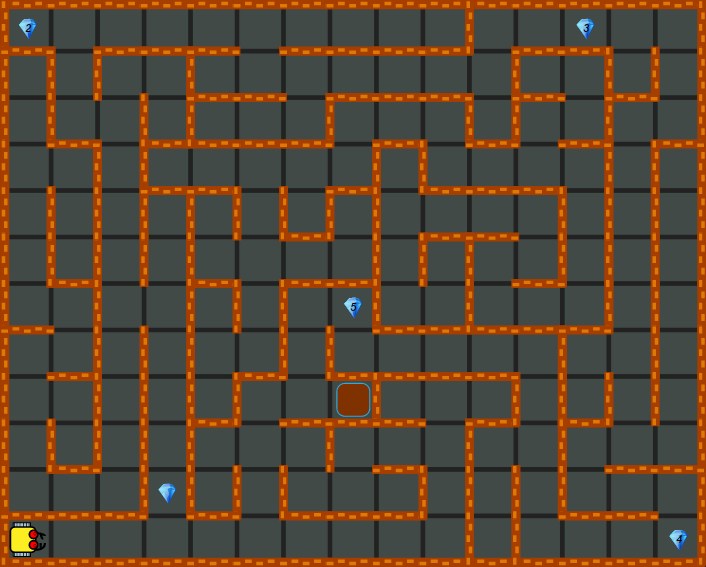
\includegraphics[height=0.4\textwidth]{img/a12.png}
\end{center}
\vspace{-4mm}
\caption{If gems are piled up, then a number is showing their amount.}
\label{fig:a12}
\vspace{-10mm}
\end{figure}
\noindent

\subsection{Gems on table}

{\em Karel has five gems in his bag. Use the buttons on the left to put the gems on the table and 
return home in time!}

\begin{figure}[!ht]
\begin{center}
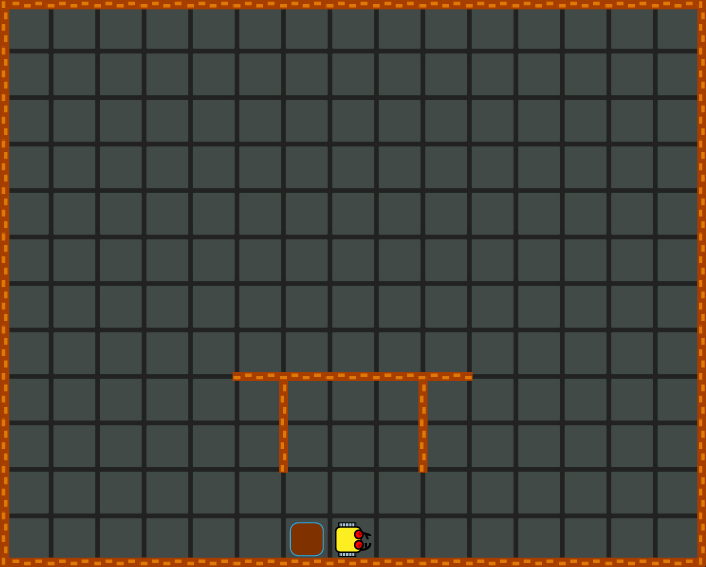
\includegraphics[height=0.4\textwidth]{img/a13.png}
\end{center}
\vspace{-4mm}
\caption{Karel needs to put five gems on the table.}
\label{fig:a13}
\vspace{-4mm}
\end{figure}
\noindent

%%%%%%%%%%%%%%%%%%%%%%%%%%%%%%%%%%%%%%%%%%%%%%%%%%%%%%%%%%%%%%%%%%%%%%%%%%%%%%%%%%%%%%%%%%

\section{Programming Mode}



\subsection{First program}

{\em Write a program that gets Karel home! Remember: Always write one command per line.}

\begin{figure}[!ht]
\begin{center}
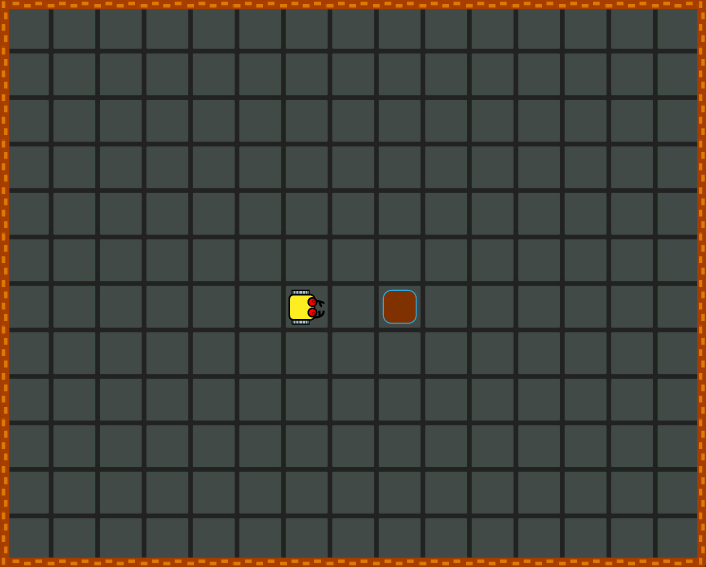
\includegraphics[height=0.4\textwidth]{img/b01.png}
\end{center}
\vspace{-4mm}
\caption{Moving Karel forward via the {\tt go} command.}
\label{fig:b01}
\vspace{-4mm}
\end{figure}
\noindent



\subsection{Three gems}

{\em Write a program for Karel to collect all gems and get home! 

\begin{figure}[!ht]
\begin{center}
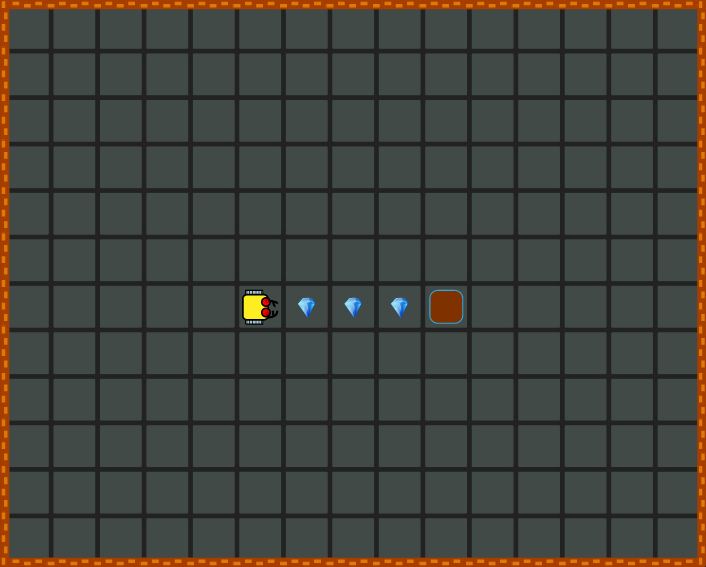
\includegraphics[height=0.4\textwidth]{img/b02.png}
\end{center}
\vspace{-4mm}
\caption{Collecting gems using the {\tt get} command.}
\label{fig:b02}
\vspace{-1cm}
\end{figure}
\newpage


\subsection{Diagonal move}

{\em Write a program for Karel to collect the gem and return home! 

\begin{figure}[!ht]
\begin{center}
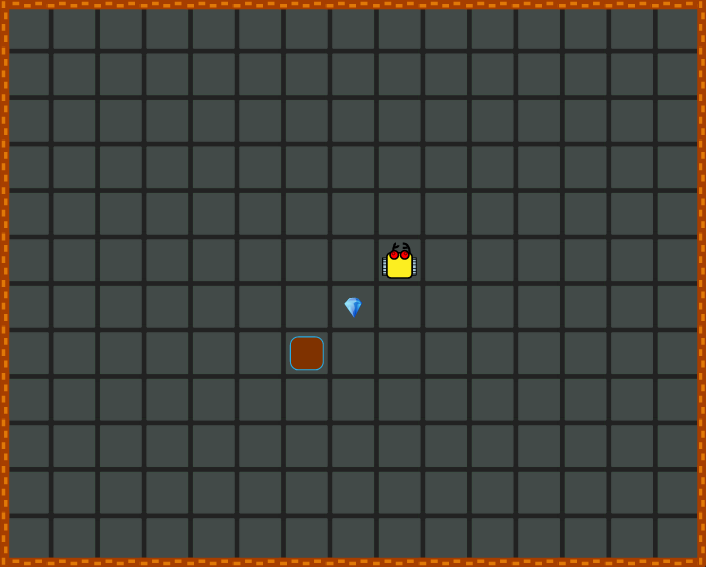
\includegraphics[height=0.4\textwidth]{img/b03.png}
\end{center}
\vspace{-4mm}
\caption{Turning to the left and to the right via the {\tt left} and {\tt right} commands.}
\label{fig:b03}
\vspace{-1cm}
\end{figure}



\subsection{Five gems}

{\em Write a program for Karel to collect all five gems and get home!}
\begin{figure}[!ht]
\begin{center}
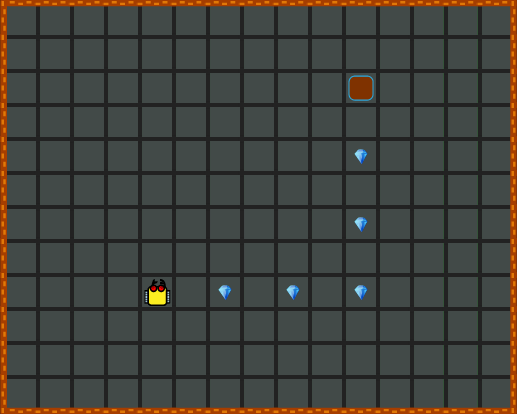
\includegraphics[height=0.4\textwidth]{img/a18.png}
\end{center}
\vspace{-4mm}
\caption{Collecting five gems.}
\label{fig:a18}
\vspace{-4mm}
\end{figure}



\subsection{Four gems}
{\em Karel needs to collect four gems and return home!}

\begin{figure}[!ht]
\begin{center}
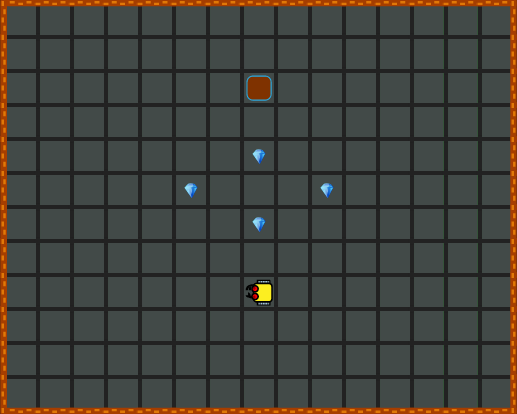
\includegraphics[height=0.4\textwidth]{img/a19.png}
\end{center}
\vspace{-4mm}
\caption{Collecting four gems.}
\label{fig:b06}
\vspace{-10mm}
\end{figure}



\subsection{Three gems}

{\em Write a program for Karel to collect all three gems and return home!}

\vspace{-3mm}
\begin{figure}[!ht]
\begin{center}
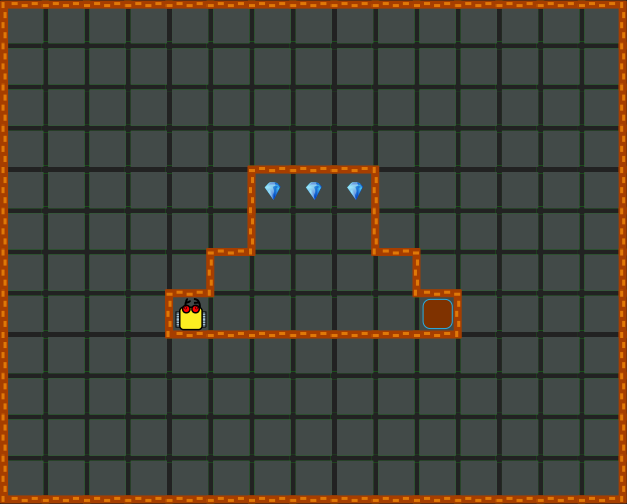
\includegraphics[height=0.4\textwidth]{img/a26.png}
\end{center}
\vspace{-4mm}
\caption{Collecting three gems.}
\label{fig:a26}
\vspace{-4mm}
\end{figure}



\subsection{Cross}

{\em Write a program for Karel to relocate the gem to the opposite 
end of the cross and return home!}

\begin{figure}[!ht]
\begin{center}
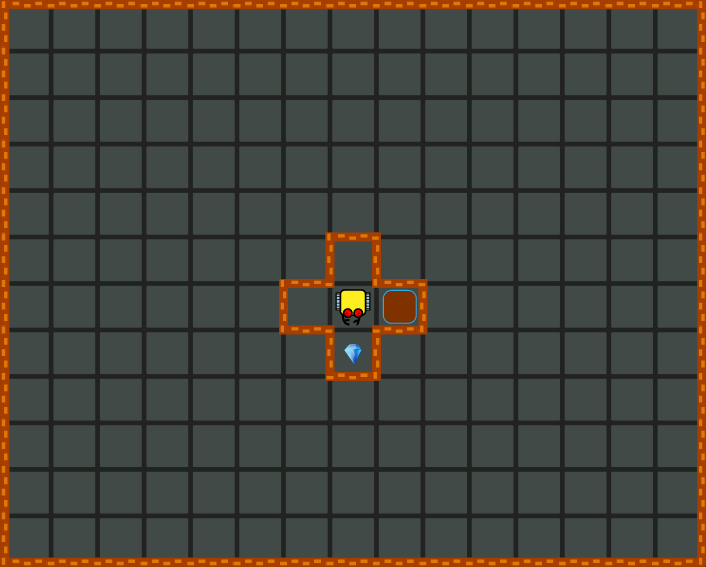
\includegraphics[height=0.4\textwidth]{img/b04.png}
\end{center}
\vspace{-4mm}
\caption{Relocating a gem requires both {\tt get} and {\tt put} commands.}
\label{fig:b04}
\vspace{-1cm}
\end{figure}

%%%%%%%%%%%%%%%%%%%%%%%%%%%%%%%%%%%%%%%%%%%%%%%%%%%%%%%%%%%%%%%%%%%%%%%%%%%%%%%%%%%%%%%%%%

\setcounter{section}{4}
\section{Counting Loop}

\subsection{Ten steps}

{\em Karel's home is ten steps away, so you could type {\tt go} ten times to get him there. 
However, knowing the {\tt repeat} command, you can do this with only {\bf two lines} of code!}

\begin{figure}[!ht]
\begin{center}
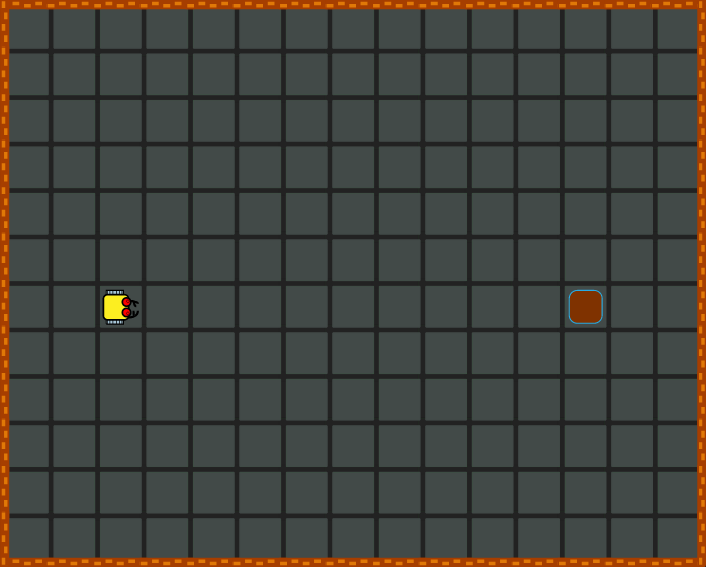
\includegraphics[height=0.4\textwidth]{img/c01.png}
\end{center}
\vspace{-4mm}
\caption{Karel gets home elegantly, using only two lines of code.}
\label{fig:c01}
\vspace{-1cm}
\end{figure}
\newpage


\subsection{Twelve gems}

{\em Karel found a pile of 12 gems! Write a program for the robot to collect all of them and get home. Your program should not be longer than {\bf eight lines} of code.}

\begin{figure}[!ht]
\begin{center}
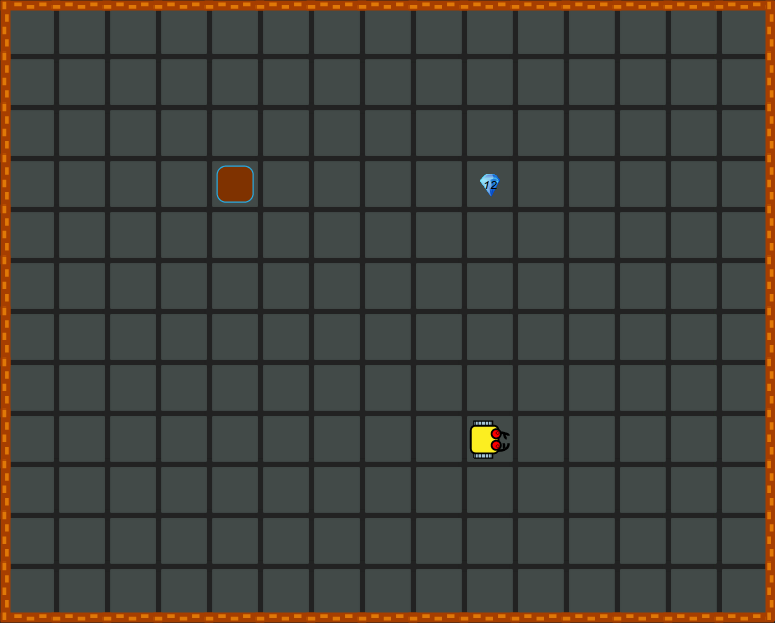
\includegraphics[height=0.4\textwidth]{img/c02.png}
\end{center}
\vspace{-4mm}
\caption{Karel found a pile of 12 gems!}
\label{fig:c02}
\vspace{-10mm}
\end{figure}
\noindent



\subsection{Feeling lucky}

{\em Karel is feeling lucky today. He wants to just step outside his house, 
turn around five times, then pick up one gem somewhere, and get back inside!}


\begin{figure}[!ht]
\begin{center}
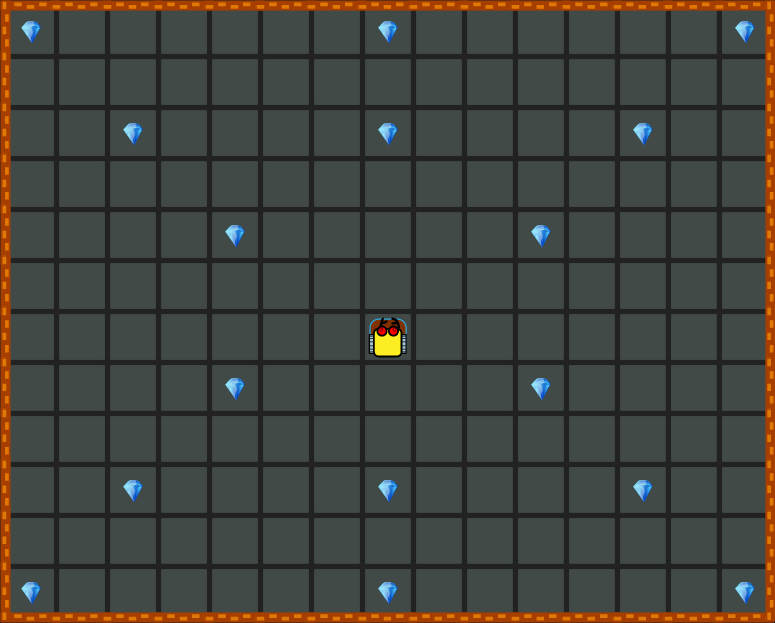
\includegraphics[height=0.4\textwidth]{img/c03.png}
\end{center}
\vspace{-4mm}
\caption{Karel is feeling lucky today.}
\label{fig:c03}
\vspace{-4mm}
\end{figure}
\noindent



\subsection{Garage sale}

{\em Karel needs to sell 10 of his oldest gems in order to make space for new ones. 
Write a program for the robot to step out of his garage, put 10 gems on the ground, 
and then turn back and get back inside! Your program should not be longer than {\bf six lines} of code.}


\begin{figure}[!ht]
\begin{center}
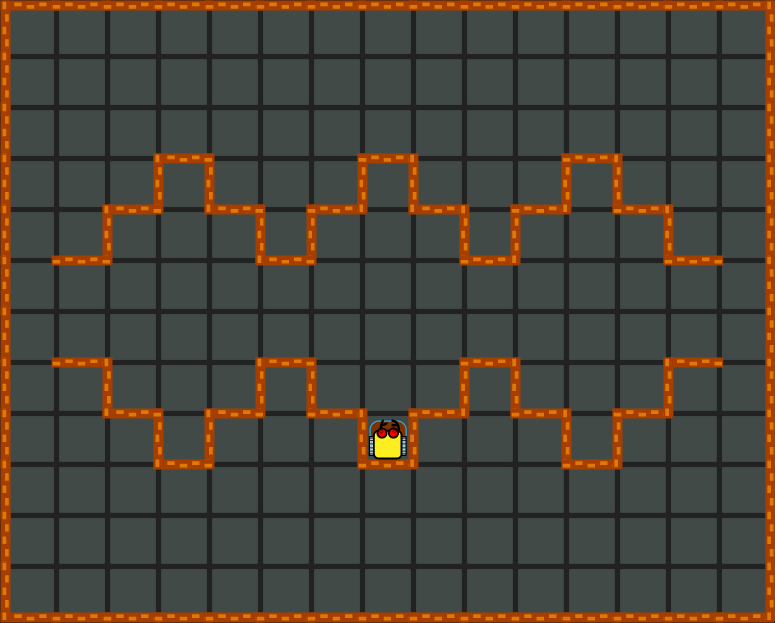
\includegraphics[height=0.4\textwidth]{img/c04.png}
\end{center}
\vspace{-4mm}
\caption{Karel is getting ready for garage sale.}
\label{fig:c04}
\vspace{-10mm}
\end{figure}



\subsection{Diamond road}

{\em Write a program for Karel to collect all nine gems and get home! 
Writing one command per line, your program should not have more 
than {\bf three lines} of code.}

\begin{figure}[!ht]
\begin{center}
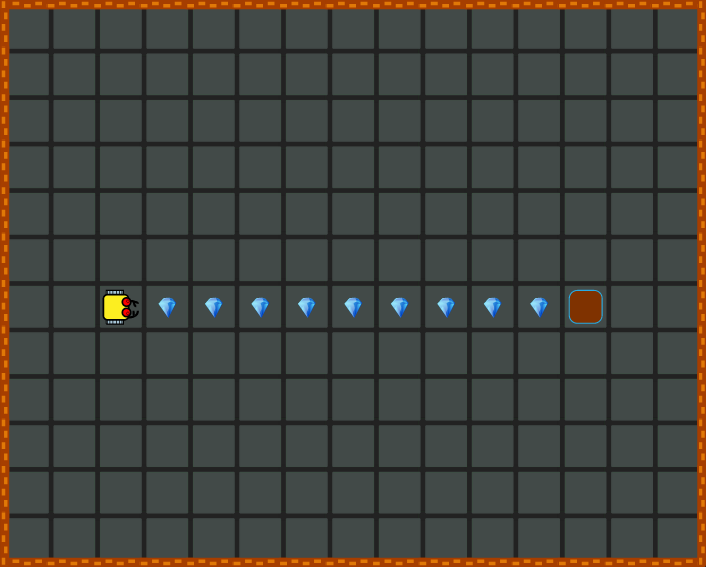
\includegraphics[height=0.4\textwidth]{img/c05.png}
\end{center}
\vspace{-4mm}
\caption{Karel is going to collect nine gems.}
\label{fig:c05}
\vspace{-10mm}
\end{figure}
\newpage



\subsection{Twenty gems}

{\em Each pile contains five gems. Write a program for Karel to collect all 
four piles and get back home. Writing one command per line, your code should not 
be longer that {\bf seven lines}.}

\begin{figure}[!ht]
\begin{center}
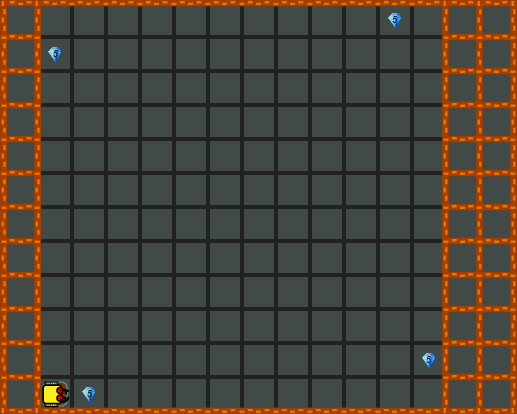
\includegraphics[height=0.4\textwidth]{img/a28.png}
\end{center}
\vspace{-4mm}
\caption{Using nested counting loops to collect four piles of gems.}
\label{fig:a28}
\vspace{-10mm}
\end{figure}

%%%%%%%%%%%%%%%%%%%%%%%%%%%%%%%%%%%%%%%%%%%%%%%%%%%%%%%%%%%%%%%%%%%%%%%%%%%%%%%%%%%%%%%%%%

\setcounter{section}{6}
\section{Conditions}

\subsection{Scattered gems}

{\em Several gems are at ramdom positions on the straight line connecting the robot and his 
home which is 10 steps away. There is at most one gem in each square. Write a program for 
Karel to collect all gems and get home. With one command per 
line, your program should have at most {\bf four lines}.}

\newpage
\begin{figure}[!ht]
\begin{center}
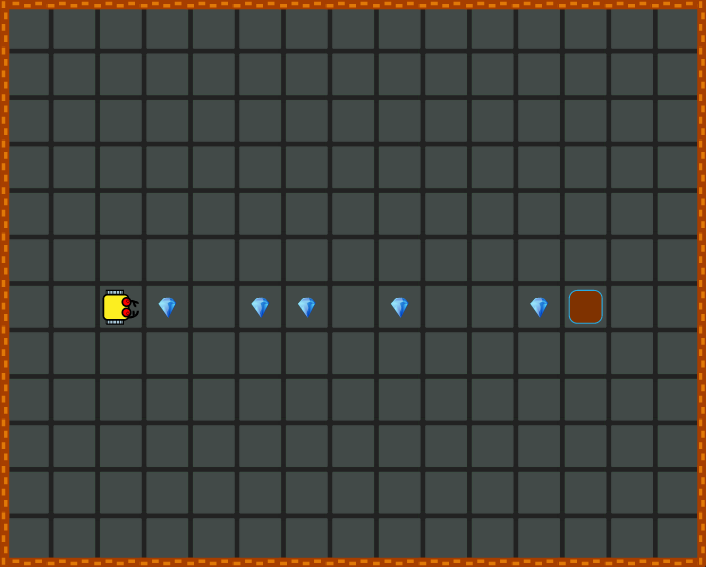
\includegraphics[height=0.4\textwidth]{img/d01.png}
\end{center}
\vspace{-4mm}
\caption{Several gems are at random positions between the robot and his home.}
\label{fig:d01}
%\vspace{-1cm}
\end{figure}
%\newpage


\subsection{Gems and stones}

{\em Karel is walking on a straight road that is covered with 
randomly placed stones and gems. His home is 14 steps away. 
Write a program for the robot to get home, avoiding stones 
and collecting all gems!}


\begin{figure}[!ht]
\begin{center}
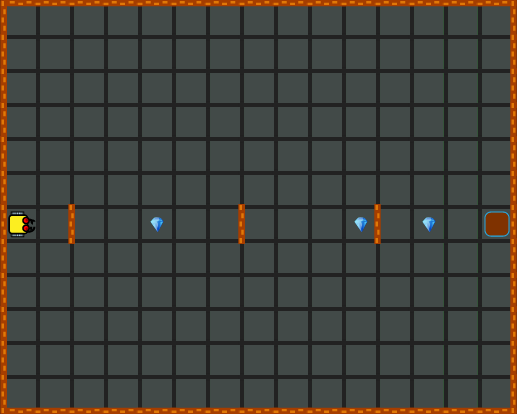
\includegraphics[height=0.4\textwidth]{img/d02.png}
\end{center}
\vspace{-4mm}
\caption{Karel is walking on a stony road.}
\label{fig:d02}
\vspace{-10mm}
\end{figure}



\subsection{Secret chest}

{\em Karel stores all his gems in a secret chest in his cellar. 
Currently, some shelves are empty. Write a program for Karel to 
inspect all shelves and put a gem where one is missing! After that, he needs to get 
home as usual. Your program should have at most 7 lines.}

\begin{figure}[!ht]
\begin{center}
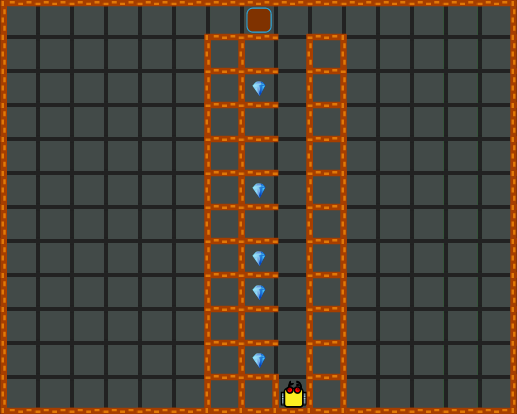
\includegraphics[height=0.4\textwidth]{img/d03.png}
\end{center}
\vspace{-4mm}
\caption{Filling empty shelves with gems.}
\label{fig:d03}
\vspace{-4mm}
\end{figure}



\subsection{Cleaning shelves}

{\em There are 11 shelves and each one is 12 squares deep. The shelves contain randomly placed gems, always at most one gem per square. Write a program for Karel to collect all gems and return home!}

\newpage

\vspace{-5mm}
\begin{figure}[!ht]
\begin{center}
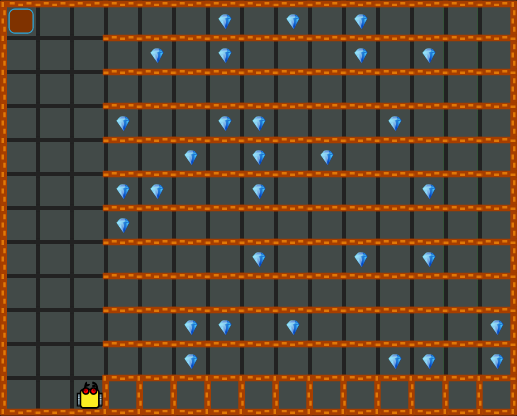
\includegraphics[height=0.4\textwidth]{img/d04.png}
\end{center}
\vspace{-4mm}
\caption{Collecting gems from 11 shelves.}
\label{fig:d04}
\vspace{-4mm}
\end{figure}

%%%%%%%%%%%%%%%%%%%%%%%%%%%%%%%%%%%%%%%%%%%%%%%%%%%%%%%%%%%%%%%%%%%%%%%%%%%%%%%%%%%%%%%%%%

\section{Conditional Loop}

\subsection{Southwest}

{\em Karel stands at a random position in the maze, facing a random direction. The maze is empty -- no walls or gems. Write a program for the robot to get to his home which is in the south-west corner! Not counting comments, your program should have 
at most {\bf nine lines}.}

\begin{figure}[!ht]
\begin{center}
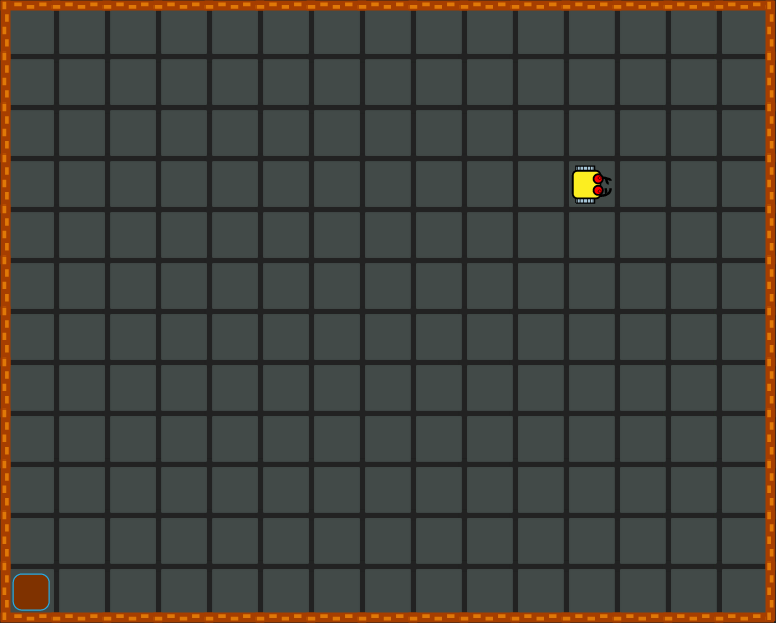
\includegraphics[height=0.4\textwidth]{img/e01.png}
\end{center}
\vspace{-4mm}
\caption{Karel only knows that his home is in the SW corner of the maze.}
\label{fig:e01}
\end{figure}



\subsection{Hide and seek}

{\em Karel's friends are hiding. To find them, he has to straight ahead 
and whenever he finds a gem, he has to collect it, 
turn left, and keep walking. Eventually, they said, he will get to the place 
where they are. Write a program for Karel to find his friends!}


\begin{figure}[!ht]
\begin{center}
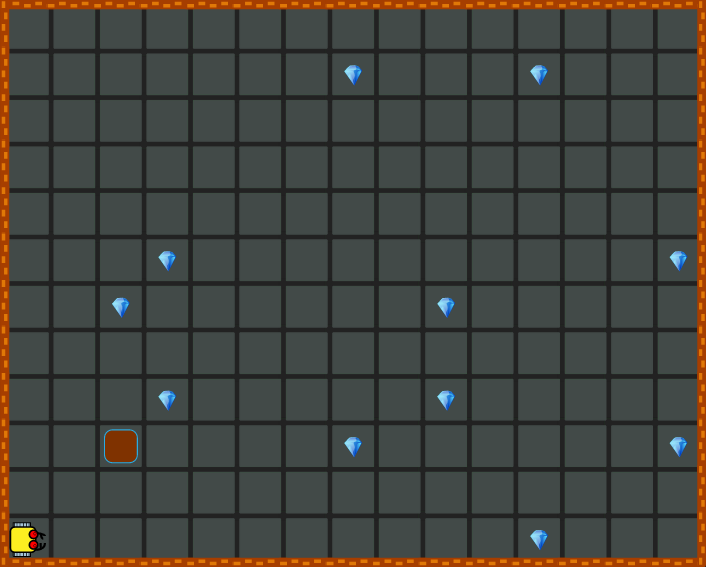
\includegraphics[height=0.4\textwidth]{img/e02.png}
\end{center}
\vspace{-4mm}
\caption{Karel plays hide-and-seek with his friends.}
\label{fig:e02}
\end{figure}



\subsection{Other side}

{\em Karel stands next to a straight wall of random length. The wall is not touching the border of the maze. The robot's home is somewhere on the other side of it but he does not know exactly where. Write a program for the robot to get there!}

\begin{figure}[!ht]
\begin{center}
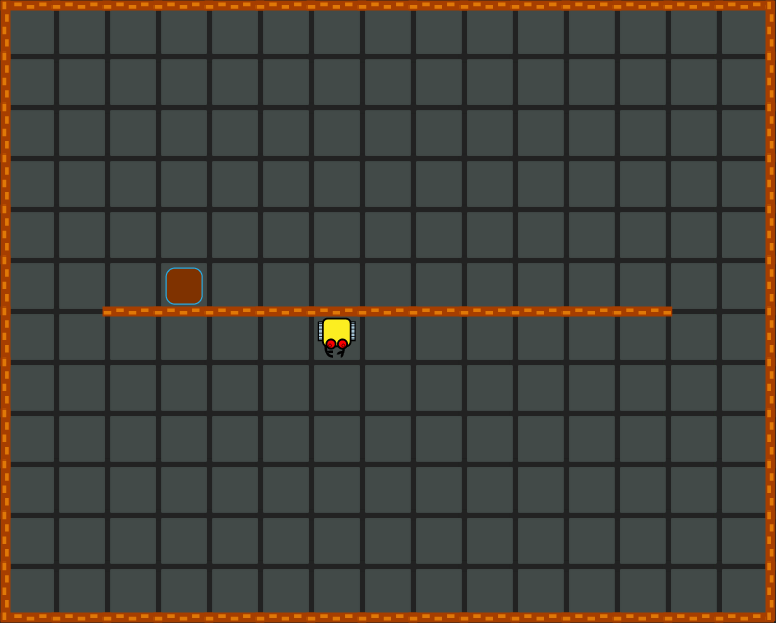
\includegraphics[height=0.4\textwidth]{img/e03.png}
\end{center}
\vspace{-4mm}
\caption{Karel knows that his home is somewhere on the other side of the wall.}
\label{fig:e03}
\end{figure}

\newpage

\subsection{Spiral}

{\em Write a program for Karel to get home. Your program should not have more than {\bf four lines}.}

\begin{figure}[!ht]
\begin{center}
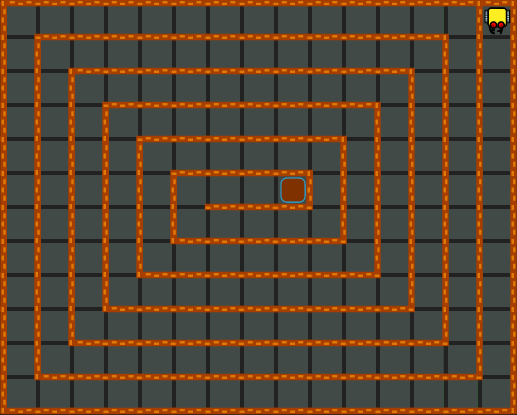
\includegraphics[height=0.4\textwidth]{img/e04.png}
\end{center}
\vspace{-4mm}
\caption{This time, Karel's home is in a spiral maze.}
\label{fig:e04}
%\vspace{-10mm}
\end{figure}



\subsection{Spiral II}

{\em Write a program for Karel to get home, collecting all the randomly placed 
gems on the way. There may be multiple gems in some squares. 
Your program should not have more than {\bf six lines}.}

\begin{figure}[!ht]
\begin{center}
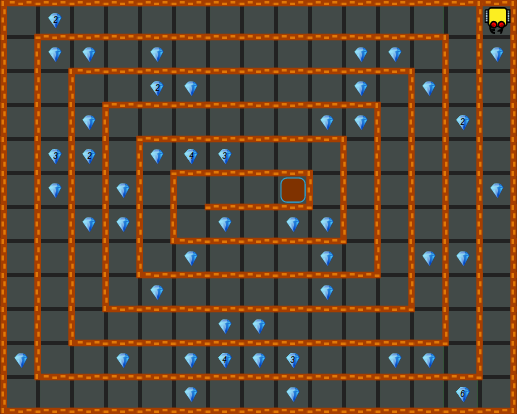
\includegraphics[height=0.4\textwidth]{img/e05.png}
\end{center}
\vspace{-4mm}
\caption{Karel needs to get home, collecting all the gems on the way.}
\label{fig:e05}
%\vspace{-10mm}
\end{figure}



\subsection{Skyline}

{\em Karel stands in the south-west corner of the maze, facing east. There 
is an array of randomly high poles and between some of them, there is a gem
on the ground. Write a program for the robot to collect all gems and get 
home!}

\newpage

\begin{figure}[!ht]
\begin{center}
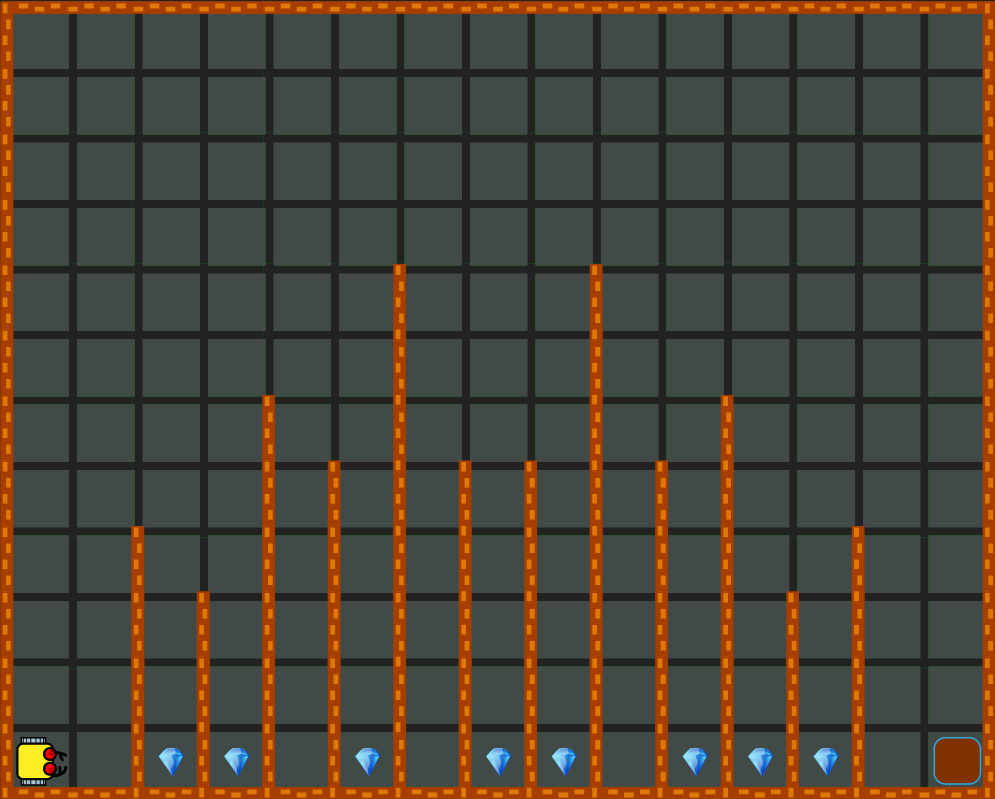
\includegraphics[height=0.4\textwidth]{img/e06.png}
\end{center}
\vspace{-4mm}
\caption{This time Karel faces an array of randomly-high poles.}
\label{fig:e06}
%\vspace{-10mm}
\end{figure}

%%%%%%%%%%%%%%%%%%%%%%%%%%%%%%%%%%%%%%%%%%%%%%%%%%%%%%%%%%%%%%%%%%%%%%%%%%%%%%%%%%%%%%%%%%

\section{Custom Commands}

\subsection{Four stars}

{\em This time Karel has to collect four stars of gems!}\\[-7mm]

\begin{figure}[!ht]
\begin{center}
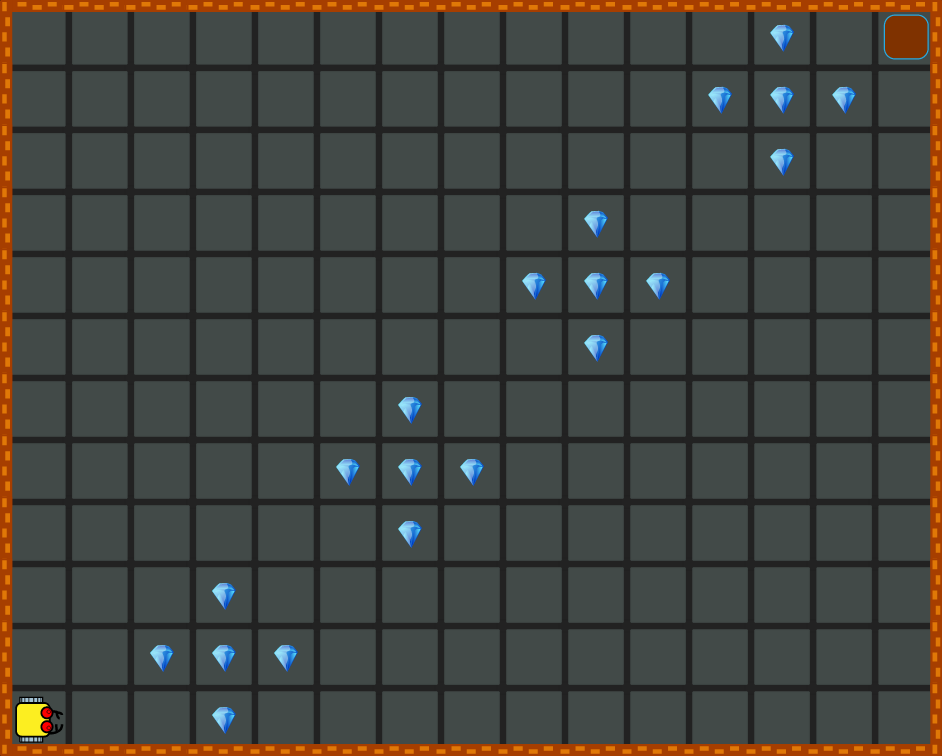
\includegraphics[height=0.4\textwidth]{img/f01.png}
\end{center}
\vspace{-4mm}
\caption{Karel needs to collect four stars of gems.}
\label{fig:f01}
\end{figure}



\subsection{Haul 36}

{\em Write a program for the robot to move the 6x6 square of gems to the 
opposite corner of the maze. The task is finished when the robot is back home.}

\begin{figure}[!ht]
\begin{center}
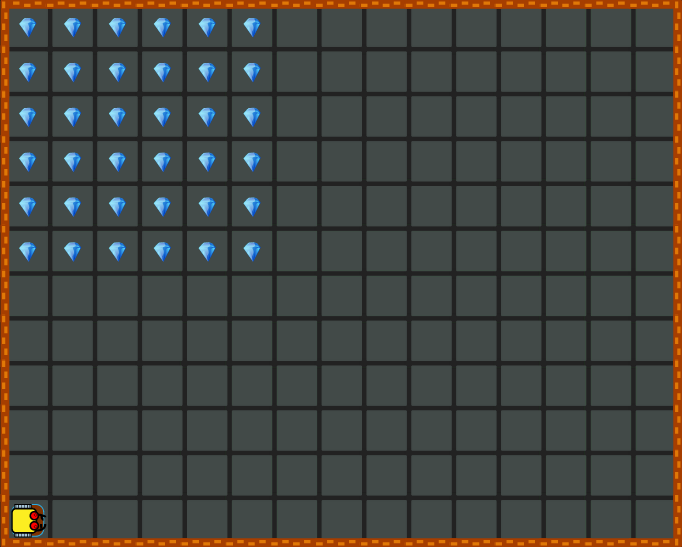
\includegraphics[height=0.4\textwidth]{img/f02.png}
\end{center}
\vspace{-4mm}
\caption{Karel needs to move the gems to the opposite corner of the maze.}
\label{fig:f02}
\end{figure}
\vspace{-1cm}



\subsection{Egg hunt}

{\em Write a program for Karel to search all cells and collect all eggs (gems) that he can find. The task is finished when the robot is back home.}


\begin{figure}[!ht]
\begin{center}
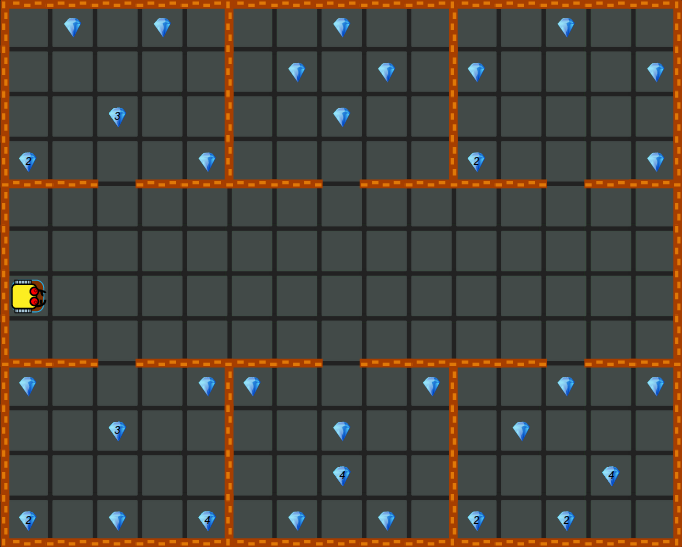
\includegraphics[height=0.4\textwidth]{img/f03.png}
\end{center}
\vspace{-4mm}
\caption{Easter is here, Karel is on egg hunt!}
\vspace{-1cm}
\label{fig:f03}
\end{figure}
\newpage


\subsection{Blind carpenter}

{\em Karel is a blind carpenter who needs to install windows (gems) into a newly built house. All he knows is that the house is a rectangle and that each window is exactly one tile large, But he can't see where the openings for the windows are. Install the windows and return home!}


\begin{figure}[!ht]
\begin{center}
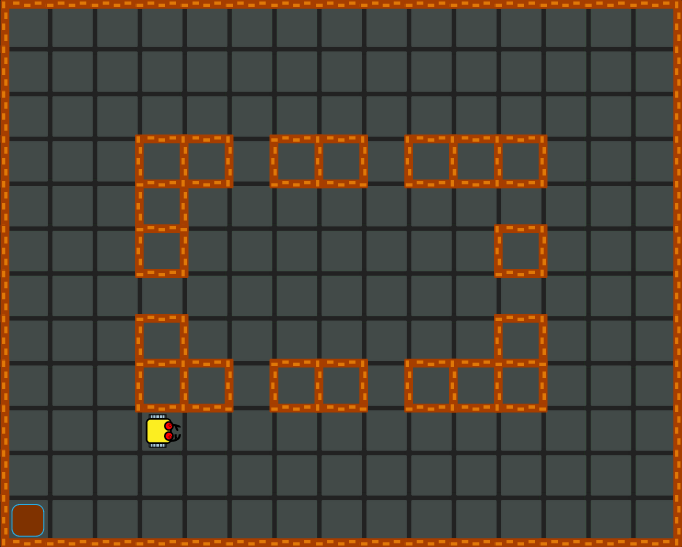
\includegraphics[height=0.4\textwidth]{img/f04.png}
\end{center}
\vspace{-4mm}
\caption{This time Karel installs windows.}
\label{fig:f04}
\end{figure}
\vspace{-1cm}



\subsection{Pirate ship}

{\em Karel is on a pirate ship! Write a program for him to collect all 
gems and run away (to his home) before the pirates are back. Here Karel 
needs to be extremely efficient to survive. Therefore, there should be 
no repeating parts whatsoever in your program!}

\begin{figure}[!ht]
\begin{center}
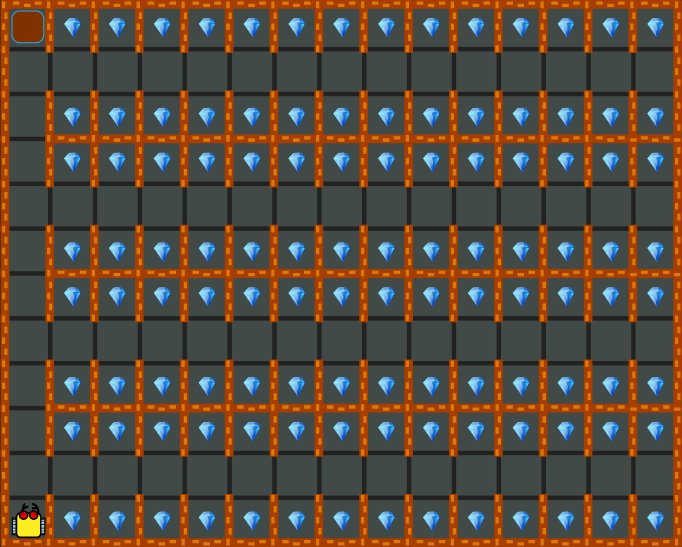
\includegraphics[height=0.4\textwidth]{img/f05.png}
\end{center}
\vspace{-4mm}
\caption{Karel found a pirate treasure.}
\label{fig:f05}
\vspace{-1cm}
\end{figure}
\newpage


\subsection{Diamond staircase}

{\em Write a program for Karel to climb the staircase, collect all gems, and 
get home. The number of steps in the staircase is random. }


\begin{figure}[!ht]
\begin{center}
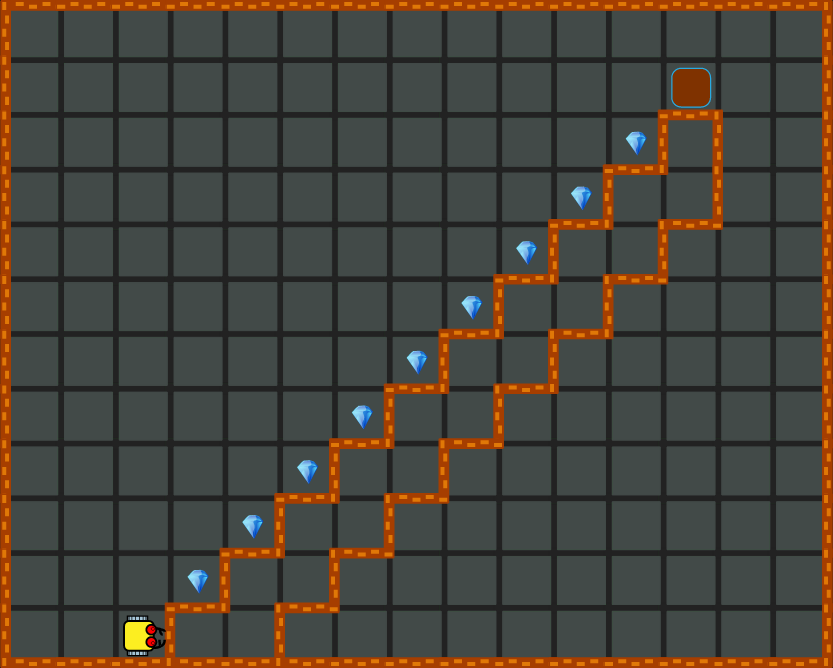
\includegraphics[height=0.4\textwidth]{img/f06.png}
\end{center}
\vspace{-4mm}
\caption{This time Karel has to do some climbing.}
\label{fig:f06}
\end{figure}



\subsection{Plucking flowers}

{\em Write a program for Karel to pluck all flowers that grow at the fence of his garden (gems), and get back home! Note two levels of repetition.}


\begin{figure}[!ht]
\begin{center}
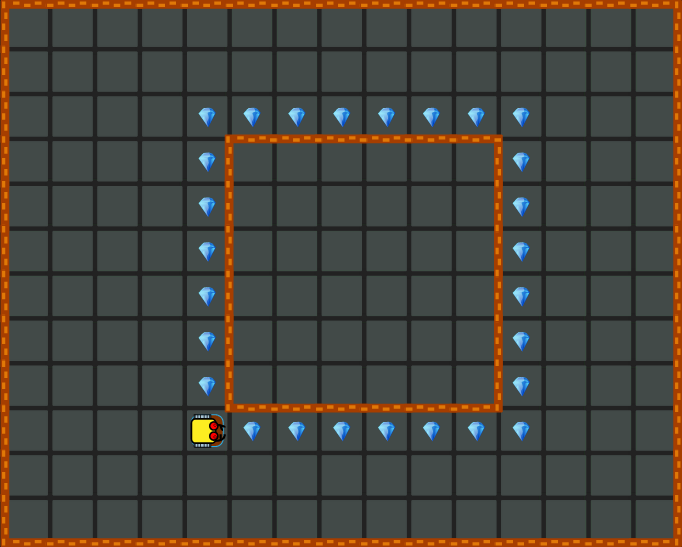
\includegraphics[height=0.4\textwidth]{img/f07.png}
\end{center}
\vspace{-4mm}
\caption{Karel is plucking flowers along his fence.}
\label{fig:f07}
\end{figure}



\subsection{Gems for friends}

{\em Karel has three gems in his bag, that he wants to give to his three friends R2, D2 and Marvin who live close by. Write a program for Karel to put a gem on the ground in the middle of each friend's home, and then return to his own home.}


\begin{figure}[!ht]
\begin{center}
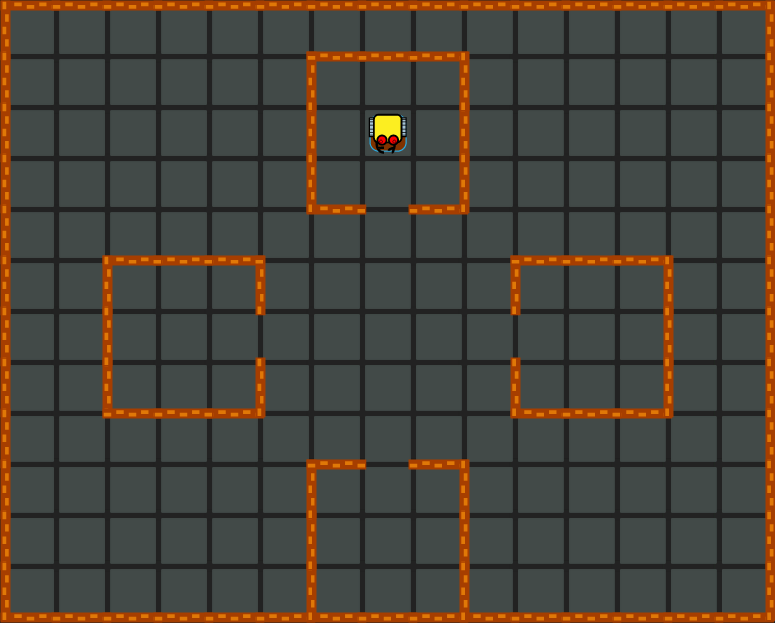
\includegraphics[height=0.4\textwidth]{img/f08.png}
\end{center}
\vspace{-4mm}
\caption{Karel is going to give gems to his three friends R2, D2 and Marvin.}
\label{fig:f08}
\vspace{-10mm}
\end{figure}



\subsection{Diamond rectangle}

{\em Karel stands in front of a diamond rectangle of unknown dimensions. Write a program for the robot to walk around the rectangle, collect all gems, and get home!}


\begin{figure}[!ht]
\begin{center}
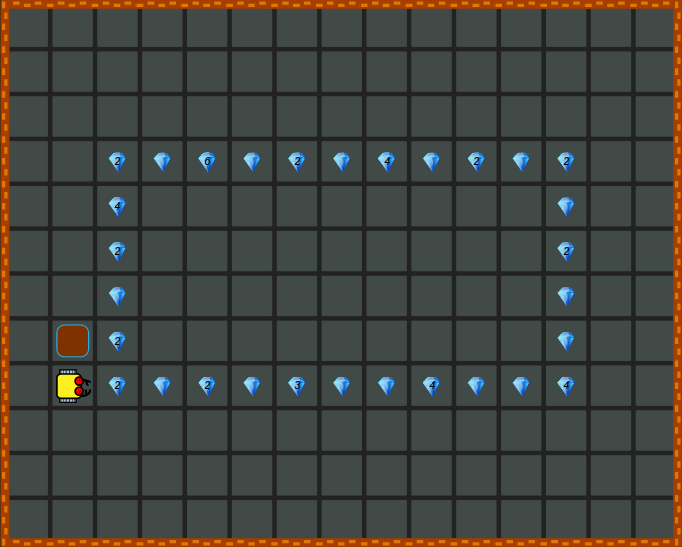
\includegraphics[height=0.4\textwidth]{img/f09.png}
\end{center}
\vspace{-4mm}
\caption{This time Karel does not know the size of the rectangle.}
\label{fig:f09}
\end{figure}
\vspace{-1cm}



\subsection{\ \ Gem jam}

{\em In this maze, gems are distributed randomly along the walls. Otherwise 
the maze is empty. Karel's home is in the south-west corner, and the robot 
stands on the right of it, facing east. Write a program for Karel to collect 
all the gems and return home!}

\begin{figure}[!ht]
\begin{center}
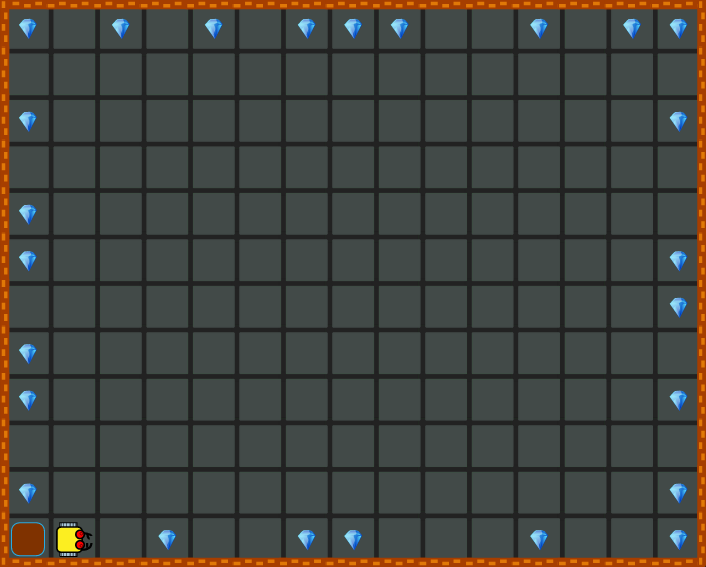
\includegraphics[height=0.4\textwidth]{img/f10.png}
\end{center}
\vspace{-4mm}
\caption{Gem Jam!}
\label{fig:f10}
\vspace{-1cm}
\end{figure}
\newpage


\subsection{\ \ The matrix}

{\em Write a program for Karel to collect all gems and enter his home!}

\begin{figure}[!ht]
\begin{center}
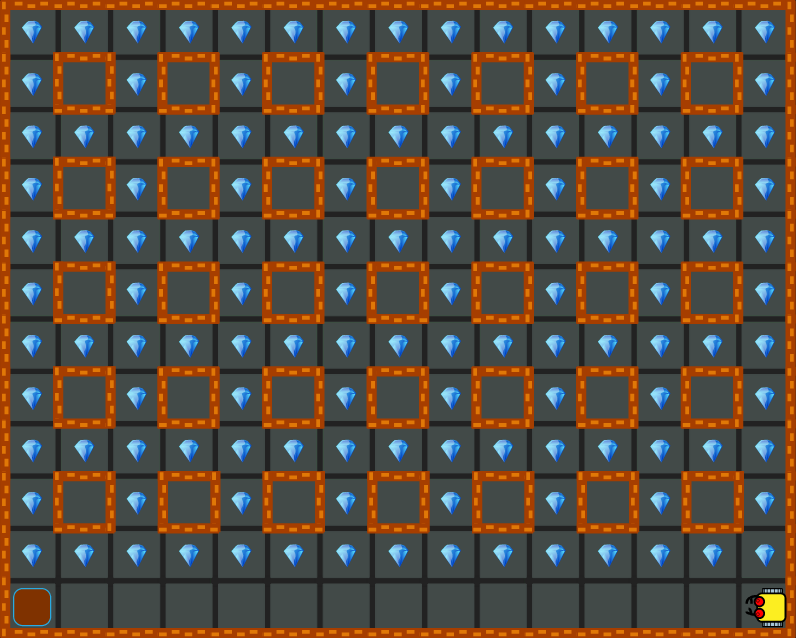
\includegraphics[height=0.4\textwidth]{img/f11.png}
\end{center}
\vspace{-4mm}
\caption{The Matrix.}
\label{fig:f11}
\end{figure}
\vspace{-1cm}



\subsection{\ \ Alcatraz}

{\em Karel is escaping from the Alcatraz prison! At the moment he is in an underground labyrinth with many random tunnels but only one of them leads to his freedom. Use the right-hand rule to find your way out!}


\begin{figure}[!ht]
\begin{center}
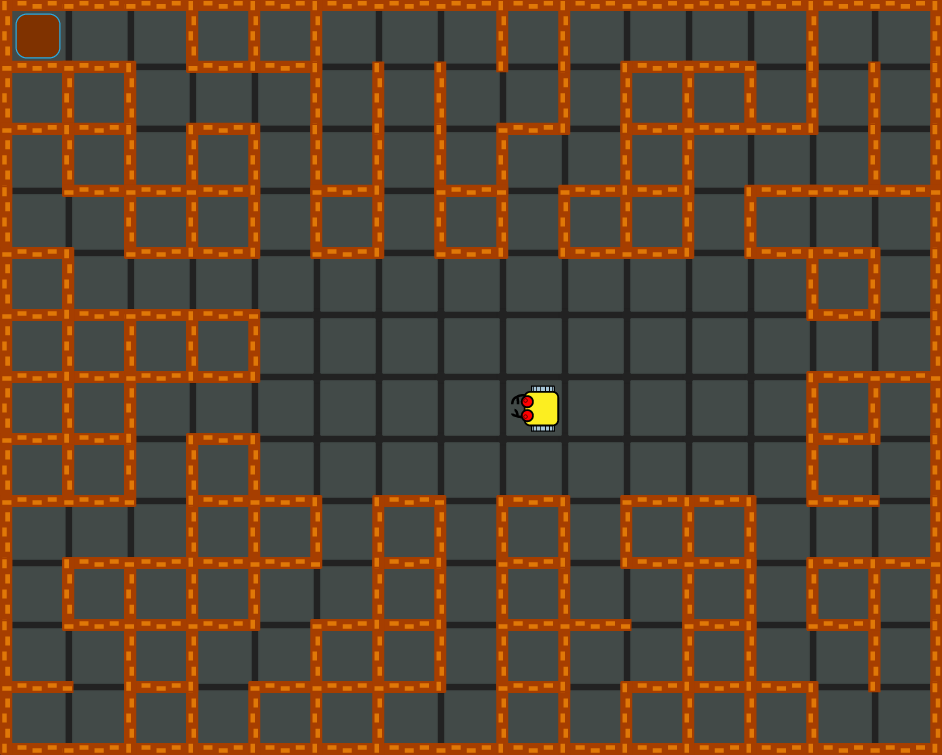
\includegraphics[height=0.4\textwidth]{img/f12.png}
\end{center}
\vspace{-4mm}
\caption{Karel is escaping from the Alcatraz prison.}
\label{fig:f12}
\vspace{-1cm}
\end{figure}
\newpage


\subsection{\ \ Border patrol}

{\em Write a program for Karel to check the perimeter of the maze using the 
right-hand rule. Do not forget to pick up all gems that you find on the way.}

\begin{figure}[!ht]
\begin{center}
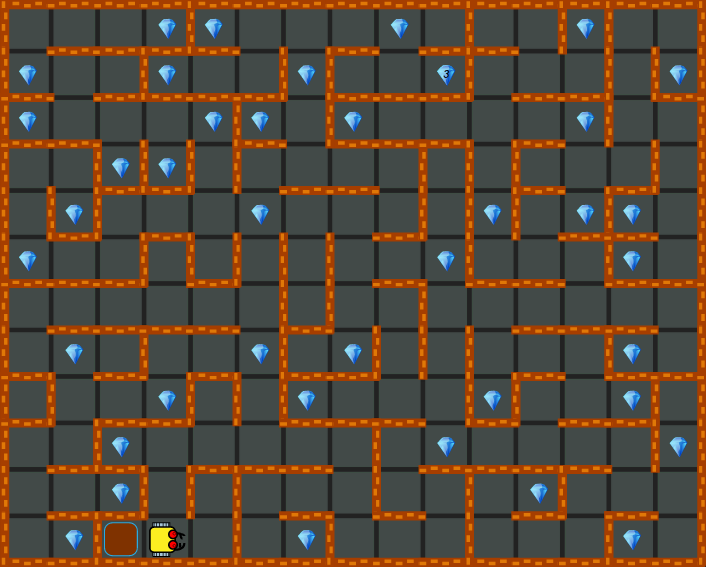
\includegraphics[height=0.4\textwidth]{img/f13.png}
\end{center}
\vspace{-4mm}
\caption{Border Patrol.}
\label{fig:f13}
\end{figure}



\subsection{\ \ Ariadne's thread}

{\em In an ancient Greek legend, princess Ariadne saved the life of her 
beloved Theseus by giving him a thread that he used to avoid getting lost 
in the maze of king Minos and kill a feared beast Minotaurus. Karel uses 
a similar technique - he leaves behind him a chain of gems that helps him 
to safely find his way back home. Your program needs to work for an 
arbitrary maze. You can assume that the string of gems is continuous 
and that it does not contain any loops.}

\newpage

\begin{figure}[!ht]
\begin{center}
\includegraphics[height=0.4\textwidth]{img/f14.png}
\end{center}
\vspace{-4mm}
\caption{Maze of king Minos, home of the beast Minotaurus.}
\label{fig:f14}
\end{figure}

%%%%%%%%%%%%%%%%%%%%%%%%%%%%%%%%%%%%%%%%%%%%%%%%%%%%%%%%%%%%%%%%%%%%%%%%%%%%%%%%%%%%%%%%%%

\section{Recursion}

\subsection{Cheese please}

{\em Karel's favorite way to eat cheese is to peel one edge at a time. His brick of 
cheese is represented by a rectangle of gems. The rectangle has random dimensions
and the robot's initial position is at one of the corners, as shown in Fig. \ref{fig:g01}.
Write a recursive algorithm for the robot to eat all the cheese and return home!
 }
\begin{figure}[!ht]
\begin{center}
\includegraphics[height=0.4\textwidth]{img/g01.png}
\end{center}
\vspace{-4mm}
\caption{Karel is eating cheese.}
\label{fig:g01}
\vspace{-1cm}
\end{figure}
\newpage


\subsection{Speleologist}

{\em Karel stands at the entrance to a cave and wants to explore it. Write a recursive program for the robot to descend the staircase to the bottom, return back, and enter his home! The number of steps in the staircase is random.}
\begin{figure}[!ht]
\begin{center}
\includegraphics[height=0.4\textwidth]{img/g02.png}
\end{center}
\vspace{-4mm}
\caption{Karel became a speleologist.}
\label{fig:g02}
\end{figure}
\vspace{-1cm}



\subsection{Homage to lemmings}

{\em  Karel has many gems in his bag, and he needs to build a heap shown in Fig. \ref{fig:g03} before he can 
enter his home. Use recursion.}

\begin{figure}[!ht]
\begin{center}
\includegraphics[height=0.4\textwidth]{img/g03.png}
\end{center}
\vspace{-4mm}
\caption{Karel needs to build a heap of gems before he can get home.}
\label{fig:g03}
\vspace{-1cm}
\end{figure}
\newpage


\subsection{Diamond tree}

{\em Karel stands under a diamond tree, with his home next to him on the the right. 
The tree is random -- at any point it can have 
a branch in the north-west or in the north-east direction (or in both). Write a recursive 
algorithm for the robot to collect all gems from the tree and get home!  }

\begin{figure}[!ht]
\begin{center}
\includegraphics[height=0.4\textwidth]{img/g04.png}
\end{center}
\vspace{-4mm}
\caption{Karel is traversing a random diamond tree.}
\label{fig:g04}
\vspace{-10mm}
\end{figure}

%%%%%%%%%%%%%%%%%%%%%%%%%%%%%%%%%%%%%%%%%%%%%%%%%%%%%%%%%%%%%%%%%%%%%%%%%%%%%%%%%%%%%%%%%%

\section{Variables and Lists}

\subsection{Accounting}

{\em Karel has an unknown number of gems in his bag. Write a function {\tt accounting} for the 
robot to count the gems and return their number. Then call the function and print the result.}

\newpage

\begin{figure}[!ht]
\begin{center}
\includegraphics[height=0.4\textwidth]{img/h01.png}
\end{center}
\vspace{-4mm}
\caption{Karel is counting his gems.}
\label{fig:h01}
\end{figure}



\subsection{Tape measure}

{\em Karel stands in a rectangular room with random dimensions. Write function {\tt measure}  
that returns a list [x, y] where 'x' and 'y' are the horizontal and vertical sizes of the room,
respectively. Call the function and print the result.}

\begin{figure}[!ht]
\begin{center}
\includegraphics[height=0.4\textwidth]{img/h02.png}
\end{center}
\vspace{-4mm}
\caption{Karel is measuring his room.}
\label{fig:h02}
\end{figure}



\subsection{Reconnaissance}

{\em Karel stands in a rectangular room with random dimensions, that contains gems at random positions. There is at most one gem in each square. Write function {\tt gems}  that returns a list of pairs [x, y] where 'x' and 'y' are the GPS coordinates of each gem. Call the function and print the result.}

\begin{figure}[!ht]
\begin{center}
\includegraphics[height=0.4\textwidth]{img/h02b.png}
\end{center}
\vspace{-4mm}
\caption{Karel is locating gems.}
\label{fig:h02b}
\end{figure}



\subsection{Orchard}

{\em Trees in Karel's orchard are represented by piles of gems. The position of trees as well as the number of apples per tree are random. Initial position of the robot is in the south-west corner, facing east. There are no walls to crash into. Write a procedure {\tt orchard} for the robot to return a list of triplets [x, y, n] with one triplet per tree, where 'x' and 'y' are the GPS coordinates and 'n' the number of apples on the tree.}

\newpage

\begin{figure}[!ht]
\begin{center}
\includegraphics[height=0.4\textwidth]{img/h03.png}
\end{center}
\vspace{-4mm}
\caption{Karel is locating trees and counting apples in his orchard.}
\label{fig:h03}
\end{figure}


\subsection{New carpet}

{\em Karel needs new carpet! His apartment has random but simple shape -- wherever 
the robot stands, when he goes north, south, east or west he will always reach exterior wall.
The initial position of the robot is at the west wall of the bottom row, facing east. 
Write a function {\tt carpet} that returns a list of triplets [x, y, n] with one triplet for each
row, starting with the bottom one, where 'x' and 'y' are the GPS coordinates of the left-most
square, and 'n' is the size of the row. }

\newpage

\begin{figure}[!ht]
\begin{center}
\includegraphics[height=0.4\textwidth]{img/h04.png}
\end{center}
\vspace{-4mm}
\caption{Karel is measuring his apartment before buying new carpet.}
\label{fig:h04}
\end{figure}

%%%%%%%%%%%%%%%%%%%%%%%%%%%%%%%%%%%%%%%%%%%%%%%%%%%%%%%%%%%%%%%%%%%%%%%%%%%%%%%%%%%%%%%%%%

\section{Logic}

\subsection{Reading numbers}

{\em Each 3x5 box contains a random integer number between 0 and 9. Write a function "readnumber" 
where Karel enters a box, determines the number in it, and returns it. Initial position of the 
robot is at the entrance of the box, facing north. The final position of the robot should be the same. 
Use this function to determine the numbers in the three boxes as shown in the screenshot. }

\newpage

\begin{figure}[!ht]
\begin{center}
\includegraphics[height=0.4\textwidth]{img/i01.png}
\end{center}
\vspace{-4mm}
\caption{Karel is learning to read numbers.}
\label{fig:g10}
\end{figure}



\subsection{Writing numbers}

{\em There is a pile of gems at the entrance of each box. The number of gems in each pile is random between 0 and 9. Write a function "writenumber" where Karel counts the gems in the pile, enters the box, and renders the number. Then use the function to render numbers in three boxes as shown in the screenshot. }

\begin{figure}[!ht]
\begin{center}
\includegraphics[height=0.4\textwidth]{img/i02.png}
\end{center}
\vspace{-4mm}
\caption{Karel is learning to write numbers.}
\label{fig:g11}
\vspace{-10mm}
\end{figure}



\subsection{Adding numbers}

This is an extra credit problem that can be solved with the help of the results 
of the previous two exercises.\\

\noindent
{\em The two upper boxes contain randomly generated numbers between 0 and 9. Karel stands at the entrance of the first box,
facing north. Write a function {\tt addnumbers} where Karel will enter each box, determine the number in it,
and then add the numbers together and return the result. Also render the result in the double-box below. 
Use the functionality developed in the previous two tasks!}


\begin{figure}[!ht]
\begin{center}
\includegraphics[height=0.4\textwidth]{img/i03.png}
\end{center}
\vspace{-4mm}
\caption{Karel is adding randomly generated numbers.}
\label{fig:g12}
\end{figure}




\subsection{Eight queens}

This is an extra credit problem -- quite a tough one. Check Wikipedia for 
"eight queens puzzle". \\

\noindent
{\em Karel stands on an 8 x 8 chess board along with eight queens (the gems). Recall that a chess queen dominates its row, its column, as well as both diagonals that pass through her position. Nothing may stand in these fields or she will destroy it. Currently, some queens are threatening each other. Write a program for Karel to correct the positions of the queens in such a way that none of them is threatened. Your program should be able to do it for any initial distribution of the queens. }

\begin{figure}[!ht]
\begin{center}
\includegraphics[height=0.4\textwidth]{img/i04.png}
\end{center}
\vspace{-4mm}
\caption{The famous eight queens problem.}
\label{fig:g14}
\end{figure}




\subsection{Bubble sort}

This is an extra credit problem -- first learn the BubbleSort algorithm,
for example using Wikipedia. \\

\noindent
{\em Karel stands in front of 9 piles of gems, containing randomly between 1 and 9 gems. Two or more piles can 
be equally large. Sort the piles in such a way that the smallest pile is on the left and the largest on the 
right. Use the BubbleSort algorithm.}

\begin{figure}[!ht]
\begin{center}
\includegraphics[height=0.4\textwidth]{img/i05.png}
\end{center}
\vspace{-4mm}
\caption{BubbleSort algorithm.}
\label{fig:g13}
\end{figure}
\noindent

